\section{DISCUSSION}

\bulletpoints{
    \item Topic Sentence: Discuss the properties of the model from a numerical perspective.
    \item The constant number of solver iterations implies that the truncation error from the integrator is minimal compared to the kinematic error.
    \item The small number of solver iterations show the importance of constant runtime improvements.
    \item Although the function calls across AB methods are the same, runtime increases due to the extra workload
    \item Quaternion model provides a stabilizing effect on integrators with small stability regions (FE \& AB). RK models do not experience the same effect.
}

\commentblock{
Given the small number of solver iterations, constant runtime improvements play a crucial role for further runtime gains as can be seen by the improvements achieved by the quaternion model.
Although quaternion integration didn't affect the accuracy of RK methods significantly, a stabilizing effect can be seen on AB methods, specifically on the higher-order methods.
Furthermore, although the decreased stability region of AB methods was thought to be a concern, the constant number of solver iterations $k$ across the different integration methods implies that the truncation error introduced by the integrator is minor relative to the kinematic error of the model.
Nonetheless, AB methods experience a proportional increase in runtime in relation to the order of the method due to the additional computations required for the extrapolating polynomial.
}

\bulletpoints{
    \item Topic Sentence: Discuss how out proposed optimization techniques offer a universal approach that achieves real-time control and mentions its limitations.
    \item We achieved a 90\% reduction in runtime, with a final runtime of 120 ms or 8.3 kHz
    \item Our approach can be universally applied to any Cosserat Rod model, regardless of architecture or actuation system.
    \item Specific optimization approaches can be further enhanced by using our approach to compliment theirs
    \item Our approach may provide limited improvements with models that do not rely on standard explicit integrators and/or numerical non-linear solvers.
}

\commentblock{
Combining all the optimizations discussed above has reduced the function call count by $90\%$ achieving an average static FK model runtime of \SI{120}{\mu s} (\SI{8.3}{kHz}), qualifying its use for high frequency, real-time systems.
Given that our proposed approach focuses on numerical enhancements instead of analytical methods, it can provide universal runtime enhancements regardless of the robot's architecture or actuation system used.
Additionally, analytical approaches may experience further optimization improvements by utilizing our approach alongside the optimized model due to the non-conflicting natures of both methods \cite{RuckerWebster_ICRA_2011, OrekhovSimaan_IROS_2020}.
It is worth noting that the proposed approach may provide limited optimization gains for models that do not rely on standard explicit integrators and/or numerical non-linear solvers, although such models are uncommon in the literature \cite{Burgner-Kahrs_TRO_2015}.
}

\subsection{Numerical Proxy for Elastic Stability}

\bulletpoints{
    \item Topic Sentence: Introduce and explain the theory behind snapping and bifurcations
    \item Discuss how torsional energy causes snapping
    \item Introduce the concept of global minimas with respect to energy states
    \item Define elastic instability with respect to the relative axial angle
    \item Explain how the ODE system evolves through a bifurcation
}

\commentblock{
\begin{figure*}
\centering
\begin{subfigure}{0.49\textwidth}
    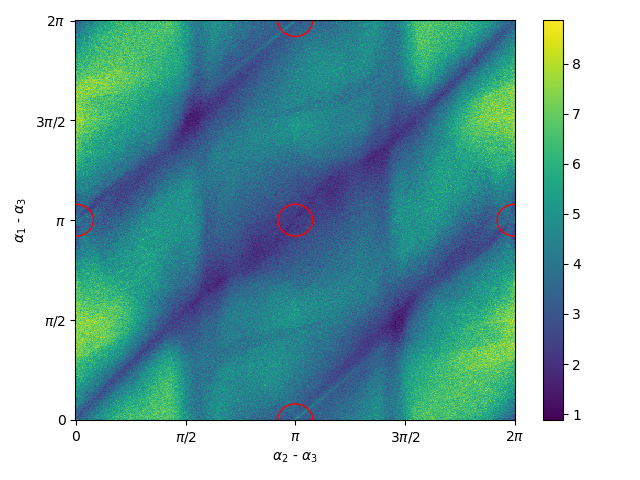
\includegraphics[width=\textwidth]{Figures/max eigen_Alpha 2 - Alpha 3-Alpha 1 - Alpha 3.png}
\end{subfigure}
\hfill
\begin{subfigure}{0.49\textwidth}
    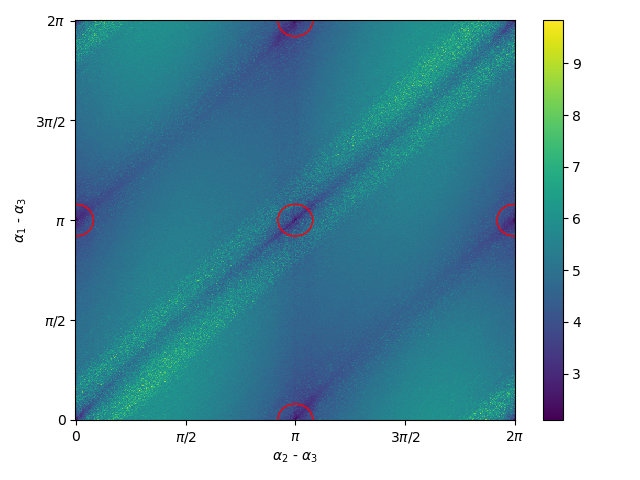
\includegraphics[width=\textwidth]{Figures/solver iterations_Alpha 2 - Alpha 3-Alpha 1 - Alpha 3.png}
\end{subfigure}
        
\caption{Mesh grids of $|\Re(\lambda_j(s))|$ (left) and solver iterations $k$ (right) with respect to the relative axial angles. $20,000,000$ random configurations were sampled. The stability equilibria points are $(0, \pi)$, $(\pi, 0)$, $(\pi, \pi)$, $(\pi, 2\pi)$, and $(2\pi, \pi)$ \cite{GilbertHendrickWebster_TRO_2016}.}
\label{fig:mesh_grids}
\end{figure*}

Snaps or bifurcations in a CTCR system occur due to built-up torsional energy, causing a sudden configuration change as the robot releases the stored tension \cite{WebsterRomanoCowan_TRO_2009}.
This snapping happens when the robot suddenly transitions from a local minimum energy state to a global minima, forcing a snap to occur \cite{WebsterRomanoCowan_TRO_2009}.
Elastic instability in a CTCR increases as the relative axial angle -- the absolute difference between the actuator's rotations -- approaches $\pi$, where instability is maximized \cite{WebsterRomanoCowan_TRO_2009, Bergeles_TRO_2015}.
After a bifurcation, the system reaches a stable equilibrium state, which typically occurs when the robot's tubes are aligned or anti-aligned \cite{GilbertHendrickWebster_TRO_2016}.
}

\bulletpoints{
    \item Topic Sentence: Discuss the experimental setup for supporting our hypothesis
    \item Static Cosserat Rod don't model dynamic energy interactions but conditioning can help us with it
    \item Equilibrium points should result in a well-conditioned system
    \item We sample 20 million configurations and generated mesh plots to visualize the conditioning wrt axial angles
}

\commentblock{
Although the static Cosserat Rod equations do not model dynamic energy interactions, they do capture the torsional energy present within the tubes.
As such, the system's elastic stability can be indirectly inferred from the ODE system's conditioning, with configurations at the equilibrium points resulting in a well-conditioned system.
To test our hypothesis, we sampled 20,000,000 random configurations and generated mesh plots of the non-linear solver's iteration count $k$ and the BVP's stiffness value $|\Re(\lambda_j(s))|$ relative to the axial angles.
These values indicate the system's conditioning, as they are influenced by the conditioning of $A$ \cite{Heath_SIAM_2018}.
}

\bulletpoints{
    \item Topic Sentence: Discuss the findings and why they support our hypothesis
    \item Areas with low stiffness overlap with equilibria
    \item Quick convergence is strongly correlated with equilibria points
    \item Coincidence with (0, 0) and (2pi, 2pi) due to default guess being correct
    \item Equilibria affects stiffness but there seems to be other stronger forces.
    \item Maybe a sentence about using the proxy planning stable paths and avoiding snapping behaviour
}

\commentblock{
As shown in Fig. ~\ref{fig:mesh_grids}, areas with low stiffness overlap with equilibrium points.
Furthermore, the non-linear solver converges the quickest around regions of equilibria, with clusters of minimal iteration counts centered exactly at the equilibrium points.
Regions surrounding points with no changes in the relative axial angles, such as $(0, 0)$ and $(2\pi, 2\pi)$, also show fast convergence due to the initial guess of zero torsional forces at the base coinciding with the correct solution.
Although elastic stability might affect stiffness, other factors seem to have a stronger influence.
This is evident from the clustering of eigenvalues at locations other than the equilibrium points.
}

\subsection{Future Work}

\bulletpoints{
    \item Topic Sentence: Discuss the jacobian A and how it needs to be investigated further
    \item Although we have jacobian A, more work needs to be done to get a reliable upper-bound.
    \item Having an upper-bound to A would give us a deeper understanding of the problem's stiffness and shed light on the elements influencing it.
    \item Also, it might helps us determine the reason of the clusters for the eigenvalues
    \item It might also explain the two-bands of abnormally large k
}

\commentblock{
Although the Jacobian matrix $A$ was introduced for the ODE system governing the BVP, an analytical upper bound for it has yet to be derived.
Such an upper bound would provide deeper insights into how the robot's parameters affect stiffness and identify which elements most significantly influence the system's conditioning.
It could also clarify the clustering behavior of the $|\Re(\lambda_j(s))|$ values and explain why they differ from solver convergence.
Furthermore, additional runtime improvements may be possible if a relationship between the optimal torsional values at the base and the eigenvalues of $A$ were to be discovered.
A thorough examination of $A$ would reveal whether such a relationship exists and how it could be exploited.
}

\bulletpoints{
    \item Topic Sentence: Discuss the proxy and how it needs to be investigated further.
    \item An in-depth investigation still needs to determine if k is a reliable indicator of stability
    \item The investigation should also examine how k could be used for planning stable paths and avoiding snapping
    \item Relationships between stiffness and the torsional forces at the base should be investigated
    \item If there is such a relation, it might provide us with a way to obtain a reliable estimate resulting in faster converging.
}

\commentblock{
Further research is necessary to determine whether the convergence count $k$ consistently serves as a reliable indicator of relative elastic stability. This investigation should explore the behavior of this numerical proxy under various scenarios, including extreme use cases, and demonstrate its practical application. The numerical proxy should also be integrated into a path planner, with the algorithm's performance evaluated in detail. If the numerical proxy proves reliable, it could be leveraged for real-time path planning and the avoidance of snapping behavior \cite{GilbertHendrickWebster_TRO_2016}.
}